\section{Preliminary Models}
\subsection{Daimler Models}

\subsubsection*{Introduction}





\subsubsection*{The static OOBN}


\subsubsection*{The dynamic OOBN}
The above described static OOBN is able to detect a maneuver 0.6s before execution. The goal is to extend the prediction horizon for manoeuvre recognition at least to 1-2 seconds (max. 4-5 seconds ahead) before the actual lane marking crossing, which is of advantage for the adaptive cruise control. Most precisely, and as indicated in the Use Case 8 on the Requirement Analysis,  the area under the ROC curve (AUC) should be greater than 0.96 for 1 second and greater than 0.9 for 2 seconds. 

Figure [timedetection] shows the evolution on time for velocity and offset in an EGO\_CutOut manoeuvre. The vertical bar indicates the moment in which the manoeuvre has been recognised by the static OOBN. By taking the temporal properties of the data into account on the model, we should be able to predict the manoeuvre earlier on time.

Each manoeuvre can be considered as a process, developing in time, i.e., as data stream given by a time sequence of the transition from lane follow into lane change manoeuvre. The dynamic extension involves copies of the static OOBN for different number of time steps in the time window (e.g. see Fig. \ref{Figure:daimlerLEdyn} where the two top nodes are temporal clone defining the share belief state between consecutive time steps creating a first order Markov process), if also the requirement on earlier prognostics of maneuver is to be satisfied. 

\begin{figure}
\begin{center}
\caption{\label{Figure:daimlerLEdyn}Daimler Temporal Model}
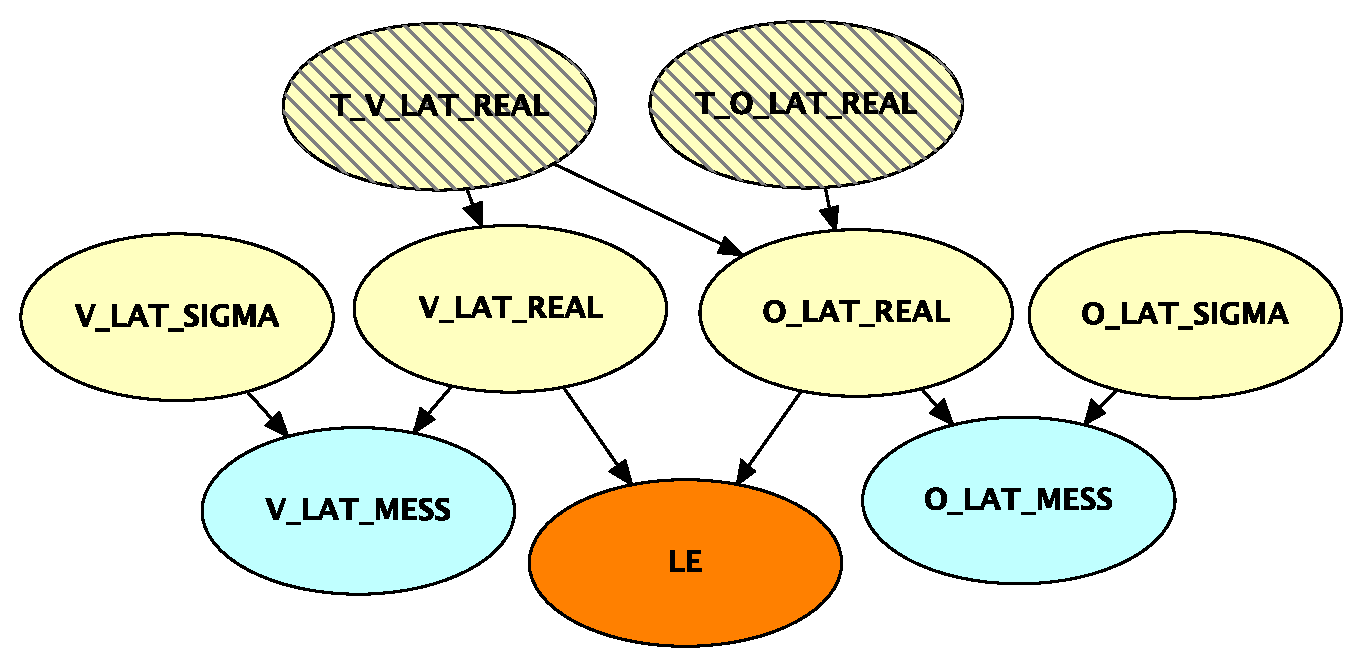
\includegraphics[scale=0.5]{./figures/LEdyn}
\end{center}
\end{figure}


\begin{enumerate}
\item \textbf{Dynamics on Lateral Evidence (LE)}
A good starting point to model the dynamics of the data involves the variables that capture the lateral evidence for the different vehicles, given its relevance and simplicity. 
The dynamic BN (DBN) incorporates the trend of change for the real values, where their physics relations are represented as causal dependencies between the time steps $dt$, e.g. in Fig. \ref{Figure:daimlerLEdyn} the transition function of O\_LAT at time $t$, O(t), is modeled as a Gaussian distribution. Its mean is affected by O(t-1), and by V\_LAT at time $t-1$, $v(t-1)$:

\begin{equation}
O(t) =O(t-1) +v(t-1)�dt +N
\end{equation}

where $N$ denotes a white noise $N(0,\sigma^2)$ due to possible acceleration term $(a�dt2)/2$, which is assumed to be small for a time step in the order of $102$ milliseconds.

The shaded nodes represent the development of the real values of observations over several time steps in the time window. Thus, their trend estimation contributes to the prediction of probability of transition from a lane follow to a lane change manoeuvre.

A DBN induces a number of constraints on the compilation of the network into a computational structure. One constraint relates to transferring the belief state from one time slice to the next where the belief state is the probability distribution over the variables shared by neighbouring time slices. In general, the belief state is transferred as a joint distribution. This means that approximate methods \cite{BoyenKoller} may have to be considered for meeting the requirements of the target platform.


\item \textbf{New hypothesis: Relative Dynamics (REL\_DYN)}

Earlier prediction of manoeuvre intentions can be achieved even before any development of the trend for lateral evidence LE has been observed. A first indication of possible lane change intention can be observed through the relative dynamics between one vehicle (host or object) and the vehicles in front of it on the same lane. Once again, the goal is to further increase the prediction horizon for manoeuvre recognition (up to 5 seconds). 

We can include qualitatively new information based on driving experience, which indicates a need for a lane change if a slower vehicle is driving in front of the own vehicle on the same lane. To continue its safe driving, the approaching vehicle should either break and reduce its speed to the speed of the vehicle in front or, alternatively,,it should change to the neighbour lane, if the neighbour lane is free and no other vehicle is approaching with a higher speed than the own vehicle. A continued safe manoeuvre (of type ``lane follow'' or ``lane change'') is modelled by estimating the TTC (TimeToCollision) to the vehicle in front (on the same lane) or to eventually approaching vehicle (on the neighbour lane). For safe manoeuvre, TTC should be bigger than 1 second, if the own vehicle wants to change to the neighbour lane or if it needs to break to ensure safe driving on the same lane (``'lane follow'') .

Figure [timedetectionRelDyn] shows the evolution on time for the velocity and distance in an EGO\_CutOut manoeuvre. The vertical bar indicates the moment in which the manoeuvre has been recognised by the static OOBN. By taking the temporal properties of the relative dynamics into account on the DBN, we should be able to predict the manoeuvre even earlier on time.

By analogy to Fig. \ref{Figure:daimlerLEdyn}, the original OOBN has been extended with the hypothesis ``relative dynamics'' (REL\_DYN), as shown in Fig.\ref{Figure:daimlerreldyn}. This BN fragment  models the hypothesis REL\_DYN with 3 states Left/Follow/RIGHT, utilising the independency assumption for the discrete variables V\_REL\_MEASSURED and X\_REL\_MEASSURED.

\begin{figure}
\begin{center}
\caption{\label{Figure:daimlerreldyn}Daimler Temporal Model with relative dynamics}
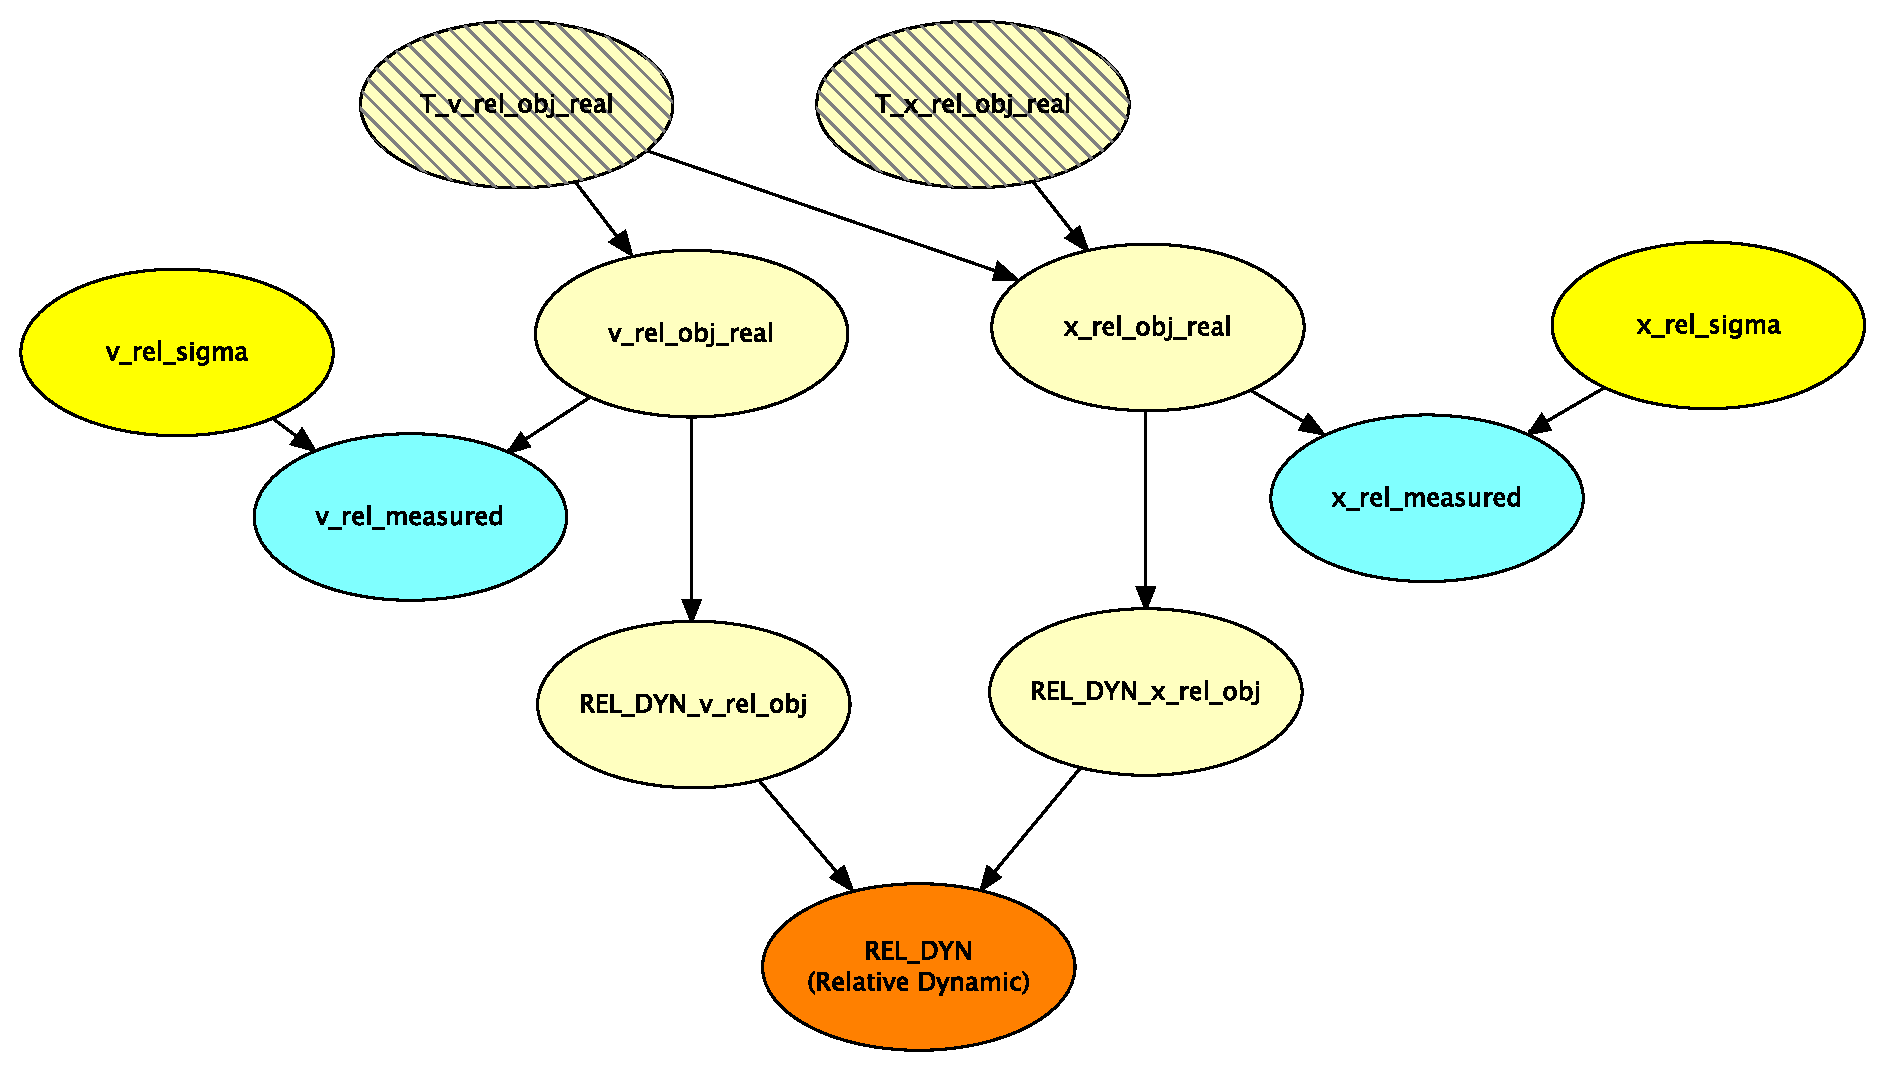
\includegraphics[scale=0.4]{./figures/reldyn}
\end{center}
\end{figure}

If we compare the structure of this network with that of Fig. \ref{Figure:daimlerLEdyn}, we can observe two additional nodes:  REL\_DYN\_V\_REL\_OBJ and REL\_DYN\_X\_REL\_OBJ. They are the results of a modelling trick to simplify the EM-learning of parameters from data for the static BN fragment.

\textcolor{red}{Note that the new REL\_DYN hypothesis introduced would require two instances in the OOBN, one for the relative dynamics of the EGO with the OBJ in front, and another one for the OBJ and another OBJ in front of it. Each REL\_DYN would indicate if the EGO and the OBJ cars are going to turn right, left or continue straight.}

\end{enumerate}
